
\documentclass[12pt]{article}
\usepackage[utf8]{inputenc}
\usepackage[brazil]{babel}
\usepackage{graphicx}
\usepackage{geometry}
\usepackage{hyperref}
\geometry{a4paper, margin=2.5cm}
\hypersetup{
    colorlinks=true,
    linkcolor=blue,
    urlcolor=blue,
    pdftitle={Relatório - Projeto de Portfólio},
    pdfauthor={Equipe: Christofer, Juan, Matheus, Pedro}
}

\title{Relatório do Projeto de Desenvolvimento de Portfólio: Leonardo Valente
Montes}
\author{
Christofer Gabriel dos Santos \\
Juan Adrian de Souza Pinheiro \\
Matheus Antoniele de Souza \\
Pedro Barbosa Ferreira
}
\date{11 de Junho de 2025}

\begin{document}

\maketitle

\tableofcontents

\newpage

\section{Introdução}

Este relatório descreve o desenvolvimento de um portfólio web realizado como parte da disciplina de Análise e Projeto de Sistemas. O cliente selecionado foi o estudante Leonardo Valente Montes, e o objetivo principal foi apresentar de forma clara suas habilidades, tecnologias dominadas e formas de contato, por meio de um portfólio moderno, funcional e responsivo.

Leonardo tem como objetivo atuar na área de Tecnologia da Informação, com interesse em desenvolvimento, suporte técnico e infraestrutura, buscando contribuir com soluções eficientes e aprender continuamente.

\section{Metodologia}

A metodologia adotada seguiu o framework proposto pela disciplina, com os marcos definidos:

\begin{itemize}
    \item \textbf{Gate A}: definição do escopo e levantamento inicial dos requisitos com o cliente.
    \item \textbf{Workshop}: revisão e alinhamento das expectativas do cliente com base na entrega inicial.
\end{itemize}

A equipe foi formada por quatro integrantes e realizou reuniões para discutir a abordagem técnica, organizar as tarefas e acompanhar o progresso. O projeto foi desenvolvido sem o uso de protótipo, utilizando um modelo já previamente criado por um dos membros da equipe, validado e aprovado pelo cliente.

\section{Desenvolvimento do Portfólio}

O portfólio foi implementado com HTML e CSS puros e pequenas funções utilizando JavaScript, com foco em uma interface moderna, limpa e funcional. As cores escolhidas foram azul escuro, tons de cinza claro e branco, de acordo com a preferência do cliente.

\subsection*{Imagem da Versão Final}

\begin{center}
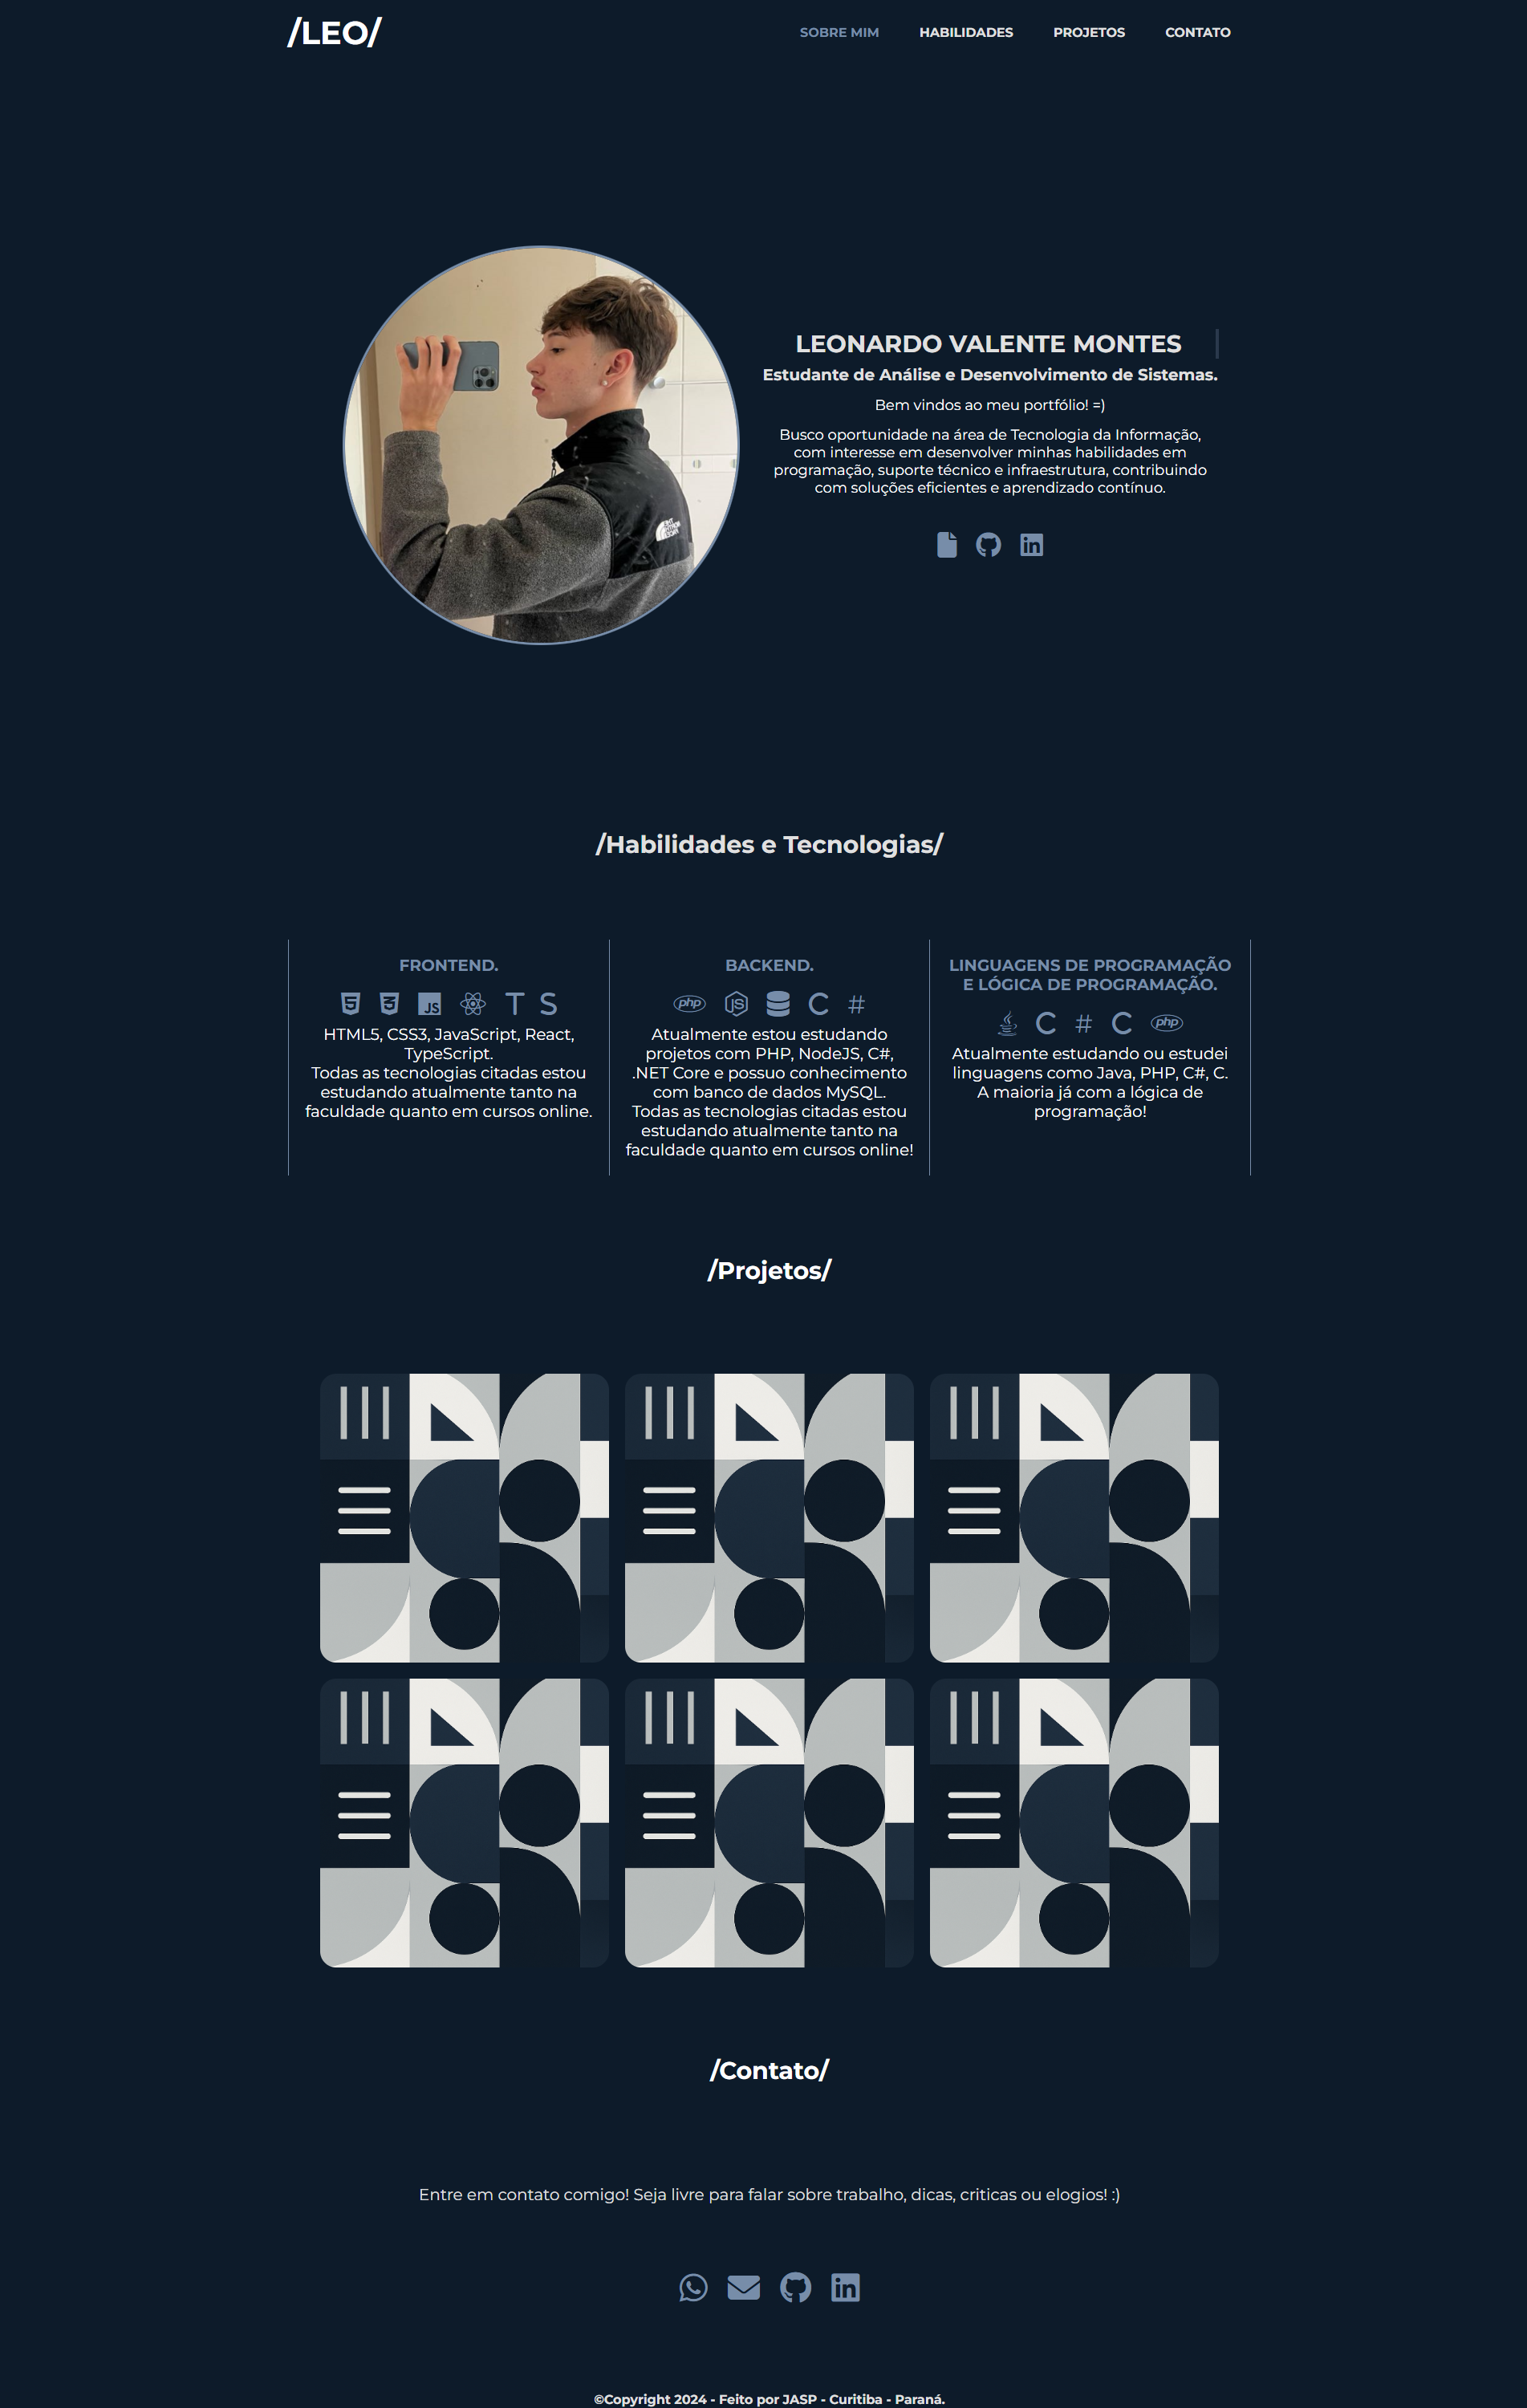
\includegraphics[width=14cm]{imagem.png}

\textbf{Figura 1:} Portfólio completo.
\end{center}
\subsection*{Funcionalidades}

\begin{itemize}
    \item Seções: Sobre mim, Habilidades, Projetos e Contato
    \item Links diretos para redes sociais (LinkedIn, GitHub, Email e WhatsApp)
    \item Layout responsivo com design visual coerente
    \item Organização clara das informações de forma sintética e navegável
\end{itemize}

\subsection*{Ferramentas Utilizadas}

Para garantir organização e clareza no desenvolvimento, utilizamos:

\begin{itemize}
    \item Trello: Gerenciamento de tarefas por colunas (Backlog, Inprog, Checking, Done)
    \item Draw.io: Criação de diagramas e fluxos visuais
    \item Visual Studio Code: Ferramenta principal para desenvolvimento e documentação
    \item GitHub: Armazenamento da versão final do projeto
\end{itemize}

\subsection*{Informações Técnicas do Cliente}

Informações Pessoais e Contato:

\begin{itemize}
    \item Nome: Leonardo Valente Montes
    \item Localidade: Campo Largo – Paraná
    \item Telefone / WhatsApp: (41) 99249-9173
    \item E-mail: valenteleonardo544@gmail.com
    \item GitHub: github.com/LeoValenteee
\end{itemize}

Formação Acadêmica:

\begin{itemize}
    \item Ensino Médio Completo
    \item Superior de Tecnologia em Análise e Desenvolvimento de Sistemas – Universidade Positivo (em andamento, noturno)
\end{itemize}

Habilidades e Técnicas:

\begin{itemize}
    \item Conhecimento em HTML e CSS
    \item Facilidade com tecnologia e aprendizado rápido
    \item Interesse nas áreas de programação, suporte e infraestrutura
\end{itemize}

\section{Conclusão}

O projeto foi concluído com sucesso dentro dos prazos estabelecidos. O cliente demonstrou satisfação com o resultado final, destacando a clareza das informações apresentadas e o visual moderno da página.

A entrega atendeu aos requisitos iniciais, e a experiência foi enriquecedora para os membros da equipe em termos de prática com tecnologias web e organização de projetos em equipe.

Apesar da implementação não ser critério de avaliação, a equipe continuará o desenvolvimento completo do portfólio para fins profissionais do cliente.

\section{Repositório no GitHub}

O repositório do projeto está disponível em:\\\href{https://github.com/JuanJASP/repositoriofinalcliente.git}{PORTFÓLIO}

\end{document}
